\documentclass[border=6pt]{standalone}
\usepackage{tikz}
\usetikzlibrary{arrows.meta,positioning}
\begin{document}
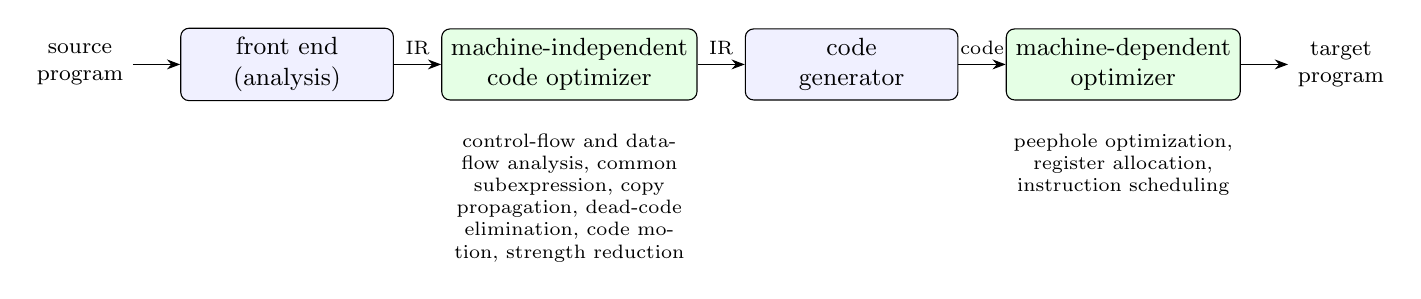
\begin{tikzpicture}[>=Stealth,font=\small,node distance=0.6cm,
 blk/.style={draw,rounded corners=3pt,minimum width=2.7cm,minimum height=0.9cm,align=center,fill=blue!6},
 io/.style={align=center,font=\footnotesize}]
\node[io] (src) {source\\program};
\node[blk,right=of src] (fe) {front end\\(analysis)};
\node[blk,right=of fe,fill=green!10] (mi) {machine-independent\\code optimizer};
\node[blk,right=of mi] (cg) {code\\generator};
\node[blk,right=of cg,fill=green!10] (md) {machine-dependent\\optimizer};
\node[io,right=of md] (tgt) {target\\program};
\draw[->] (src) -- (fe);
\draw[->] (fe) -- node[above,font=\scriptsize]{IR} (mi);
\draw[->] (mi) -- node[above,font=\scriptsize]{IR} (cg);
\draw[->] (cg) -- node[above,font=\scriptsize]{code} (md);
\draw[->] (md) -- (tgt);
\node[font=\scriptsize,align=center,below=0.3cm of mi,text width=3cm] {control-flow and data-flow analysis, common subexpression, copy propagation, dead-code elimination, code motion, strength reduction};
\node[font=\scriptsize,align=center,below=0.3cm of md,text width=3cm] {peephole optimization, register allocation, instruction scheduling};
\end{tikzpicture}
\end{document}
